\documentclass[sigconf]{acmart}
\usepackage[slantfont,boldfont]{xeCJK}
\setCJKmainfont{SimSong}

%%
%% \BibTeX command to typeset BibTeX logo in the docs
\AtBeginDocument{%
  \providecommand\BibTeX{{%
    \normalfont B\kern-0.5em{\scshape i\kern-0.25em b}\kern-0.8em\TeX}}}

%%
%% end of the preamble, start of the body of the document source.
\begin{document}

%%
%% The "title" command has an optional parameter,
%% allowing the author to define a "short title" to be used in page headers.
\title{基于机器学习的推荐系统的调研}

%%
%% The "author" command and its associated commands are used to define
%% the authors and their affiliations.
%% Of note is the shared affiliation of the first two authors, and the
%% "authornote" and "authornotemark" commands
%% used to denote shared contribution to the research.

\author{尹祥琨}
\orcid{0000-0001-6417-0859}
\affiliation
{
    \institution{山东大学计算机科学与技术学院}
    \city{青岛}
    \country{山东}
}

%%
%% The abstract is a short summary of the work to be presented in the
%% article.
\begin{abstract}
  随着在线信息的数量、复杂性和动态性的不断增长,推荐系统已成为克服此类信息过载的有效关键解决方案。机器学习在语音识别、图像分析和自然语言处理方面的革命性进展引起了广泛关注。同时,最近的研究也证明了它在处理信息检索和推荐任务方面的有效性。由于其最先进的性能和高质量的推荐,将深度学习技术应用于推荐系统已经获得了动力。与传统的推荐模型相比,深度学习可以更好地理解用户的需求、物品的特征以及它们之间的历史交互。本文旨在全面回顾基于机器学习的推荐系统的研究成果,以促进推荐系统研究的创新。

  本文概述了推荐系统领域,并描述了当前一代的推荐方法,这些方法通常分为以下三个主要类别:基于内容的推荐方法、协作推荐方法和混合推荐方法。本文还描述了当前推荐方法的各种限制,并讨论了可以提高推荐能力并使推荐系统适用于更广泛应用的可能扩展。除其他外,这些扩展包括改进对用户和项目的理解、将上下文信息合并到推荐过程中、支持多标准评级,以及提供更灵活和更少侵入性的推荐类型。
\end{abstract}

%%
%% The code below is generated by the tool at http://dl.acm.org/ccs.cfm.
%% Please copy and paste the code instead of the example below.
%%
\begin{CCSXML}
  <ccs2012>
     <concept>
         <concept_id>10002951.10003317.10003347.10003350</concept_id>
         <concept_desc>Information systems~Recommender systems</concept_desc>
         <concept_significance>500</concept_significance>
         </concept>
   </ccs2012>
\end{CCSXML}
  
\ccsdesc[500]{Information systems~Recommender systems}

%%
%% Keywords. The author(s) should pick words that accurately describe
%% the work being presented. Separate the keywords with commas.
\keywords{推荐系统, 机器学习}

%% A "teaser" image appears between the author and affiliation
%% information and the body of the document, and typically spans the
%% page.

\begin{teaserfigure}
  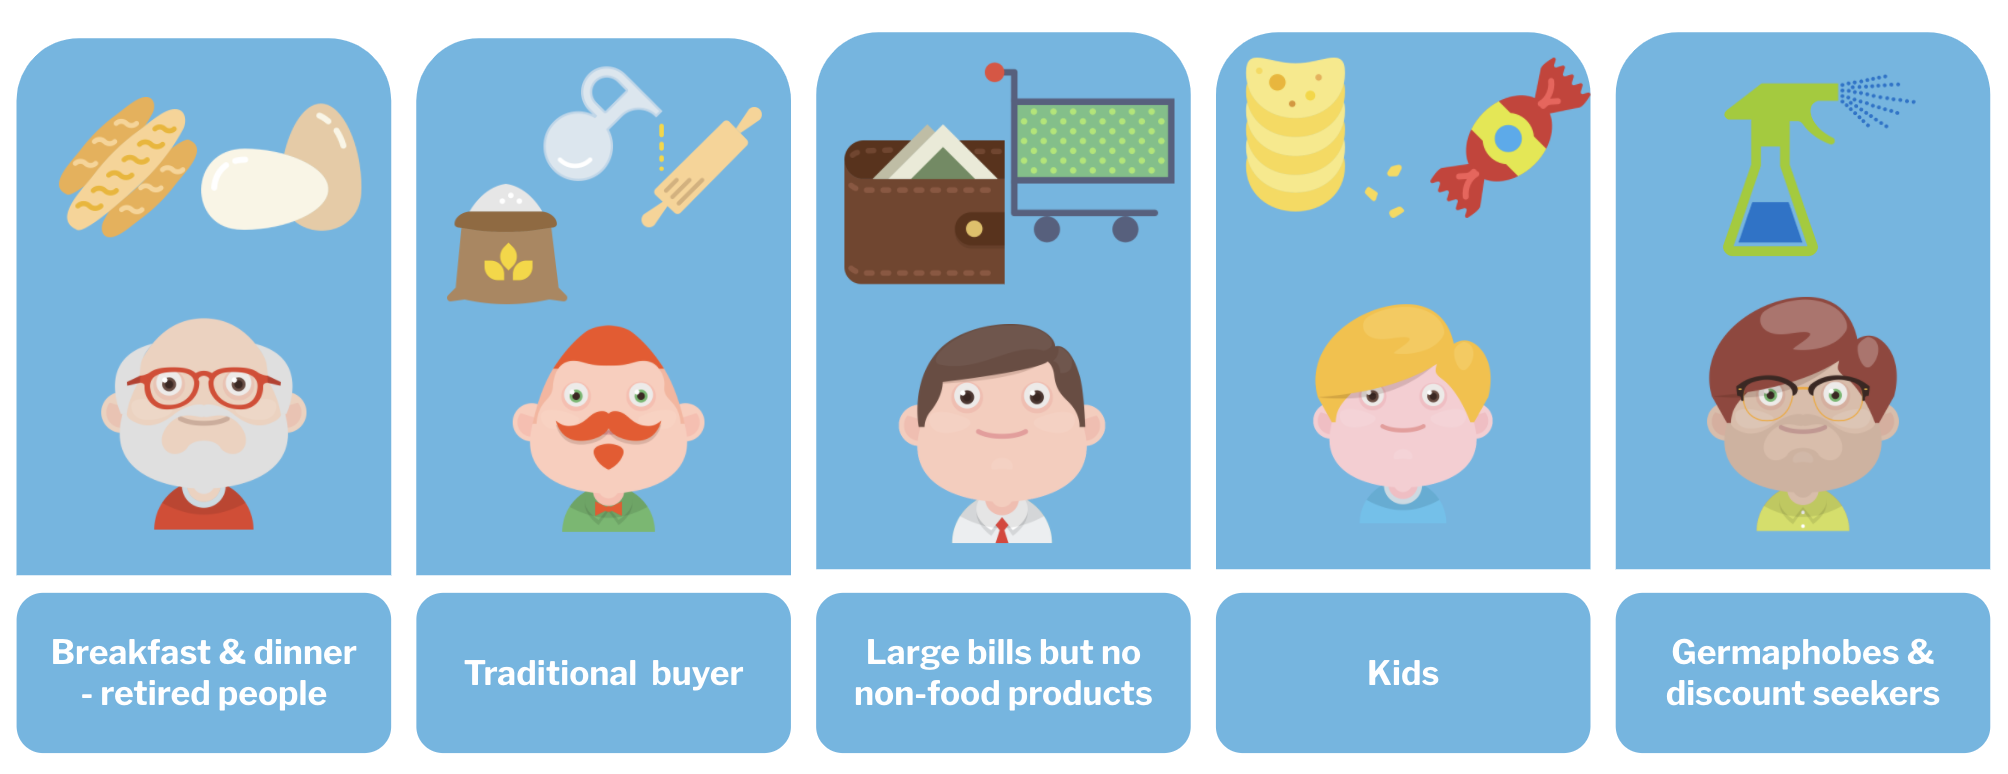
\includegraphics[width=\textwidth]{img/teaser.png}
  \caption{针对不同人的喜好进行推荐}
  \Description{针对不同人的喜好进行推荐}
  \label{fig:teaser}
\end{teaserfigure}

%%
%% This command processes the author and affiliation and title
%% information and builds the first part of the formatted document.
\maketitle

\section{Introduction}
在线可用信息的爆炸式增长经常使用户不堪重负。推荐系统是一种有用的信息过滤工具,用于指导用户以个性化的方式从大量可能的选项中发现他们可能感兴趣的产品或服务。推荐系统在各种信息访问系统中发挥着更加重要和重要的作用,以促进业务发展并促进决策过程。

一般来说,推荐列表是基于用户偏好、项目特征、用户与项目过去的交互以及一些其他附加信息(如时间和空间数据)生成的。根据输入数据的类型,推荐模型主要分为协同过滤、基于内容的推荐系统和混合推荐系统 \cite{adomavicius2005toward} 。然而,这些模型在处理数据稀疏和冷启动问题以及在不同评估指标方面平衡推荐质量方面都有其局限性


%%
%% The acknowledgments section is defined using the "acks" environment
%% (and NOT an unnumbered section). This ensures the proper
%% identification of the section in the article metadata, and the
%% consistent spelling of the heading.
\begin{acks}
  To Robert, for the bagels and explaining CMYK and color spaces.
\end{acks}

%%
%% The next two lines define the bibliography style to be used, and
%% the bibliography file.
\bibliographystyle{ACM-Reference-Format}
\bibliography{references}
  
\end{document}
\endinput
%%
%% End of file `sample-sigconf.tex'.
